\section{Scientific Communities}


The notion of community can be understood as a dense group of nodes in a network, with more edges inside than edges linking the rest of the network.  There are multiple definitions
and strategies of identifying communities and they which vary according to the context. In our context, a scientific community can be defined in terms of a large and well
established conference able to aggregates authors working in similar research topics along a considerable number of years.  Next, we describe how we build a large set of scientific
communities and present basic network evolution properties of them.


\subsection{Dataset}

In order to define a set of scientific communities to study, we focus on gathering data from DBLP\footnote{http://dblp.uni-trier.de/}~\cite{Ley:2009}, a digital library containing
more than 2.1 million publications from 1.2 million authors that provides bibliographic information on major computer science conferences and journals.  DBLP offers its entire
database in XML format, which facilitates gathering and reconstructing entire scientific communities. 

Each publication is accompanied by its title, list of authors, year of publication, and the venue of publication, i.e. the conference or journal. For the purposes of our work, we
consider a scientific community as graph in which nodes are represented by researchers and edges links co-authors of papers at the same community.  In order to define communities,
we focus on the publications from the flagship conferences of each of the ACM SIGs (Special Interest Groups).  Thus, we define a scientific community by linking people that have
co-authored a paper in a certain conference, making the flagships conferences of the ACM SIGs to serve as communities where co-authorships are formed.  We removed young SIG
conferences without enough data for a temporal analysis as well as conferences in which the entire history is not registered on DBLP, to allow us carrying temporal analyses. In
total, 26 scientific communities were considered. Table~\ref{tab:sigs_conference_period} summarizes the ACM special interest group, the flagship conference name, the period
considered (some conferences had the period reduced to avoid hiatus in the data), H-Index, number of authors, publications and editions as well as ratios extracted from these last
three measures.

\begin{table*}[!htb]
\centering
\caption{The data of DBLP of flagship conferences of ACM SIGs}
\label{tab:sigs_conference_period}
{\small
\begin{tabular}{|l|l|c|c|c|c|c|c|c|c|} \hline
SIG & Conference & Period & H-Index & Authors & Publications & Editions & Aut/Edi & Pub/Edi & Aut/Pub\\ \hline
SIGACT & STOC & 1969-2012 & 94 & 2159 & 2685 & 44 & 49.07 & 61.02 & 0.80\\ \hline
SIGAPP & SAC & 1993-2011 & 59 & 9146 & 4500 & 19 & 481.37 & 236.84 & 2.03\\ \hline
SIGARCH & ISCA & 1976-2011 & 102 & 2461 & 1352 & 36 & 68.36 & 37.56 & 1.82\\ \hline
SIGBED & HSCC & 1998-2012 & - & 846 & 617 & 15 & 56.40 & 41.13 & 1.37\\ \hline
SIGCHI & CHI & 1994-2012 & 144 & 5095 & 2819 & 19 & 268.16 & 148.37 & 1.81\\ \hline
SIGCOMM & SIGCOMM & 1988-2011 & 140 & 1593 & 796 & 24 & 66.38 & 33.17 & 2.00\\ \hline
SIGCSE & SIGCSE & 1986-2012 & 51 & 3923 & 2801 & 27 & 145.30 & 103.74 & 1.40\\ \hline
SIGDA & DAC & 1964-2011 & 98 & 8876 & 5693 & 48 & 184.92 & 118.60 & 1.56\\ \hline
SIGDOC & SIGDOC & 1989-2010 & 23 & 1071 & 810 & 22 & 48.68 & 36.82 & 1.32\\ \hline
SIGGRAPH & SIGGRAPH & 1985-2003 & 119 & 1920 & 1108 & 19 & 101.05 & 58.32 & 1.73\\ \hline
SIGIR & SIGIR & 1978-2011 & 116 & 3624 & 2687 & 34 & 106.59 & 79.03 & 1.35\\ \hline
SIGKDD & KDD & 1995-2011 & 124 & 3078 & 1699 & 17 & 181.06 & 99.94 & 1.81\\ \hline
SIGMETRICS & SIGMETRICS & 1981-2011 & 71 & 2083 & 1174 & 31 & 67.19 & 37.87 & 1.77\\ \hline
SIGMICRO & MICRO & 1987-2011 & 81 & 1557 & 855 & 25 & 62.28 & 34.20 & 1.82\\ \hline
SIGMM & Multimedia & 1993-2011 & 80 & 5400 & 2928 & 19 & 284.21 & 154.11 & 1.84\\ \hline
SIGMOBILE & MobiCom & 1995-2011 & 106 & 1151 & 480 & 17 & 67.71 & 28.24 & 2.40\\ \hline
SIGMOD & SIGMOD & 1975-2012 & 147 & 4202 & 2669 & 38 & 110.58 & 70.24 & 1.57\\ \hline
SIGOPS & PODC & 1982-2011 & 59 & 1685 & 1403 & 30 & 56.17 & 46.77 & 1.20\\ \hline
SIGPLAN & POPL & 1975-2012 & 85 & 1527 & 1217 & 38 & 40.18 & 32.03 & 1.25\\ \hline
SIGSAC & CCS & 1996-2011 & 97 & 1354 & 676 & 16 & 84.63 & 42.25 & 2.00\\ \hline
SIGSAM & ISSAC & 1988-2011 & - & 1100 & 1177 & 24 & 45.83 & 49.04 & 0.93\\ \hline
SIGSOFT & ICSE & 1987-2011 & 111 & 3502 & 2248 & 25 & 140.08 & 89.92 & 1.56\\ \hline
SIGUCCS & SIGUCCS & 1989-2011 & - & 1771 & 1593 & 23 & 77.00 & 69.26 & 1.11\\ \hline
SIGWEB & CIKM & 1992-2011 & 82 & 4978 & 2623 & 20 & 248.90 & 131.15 & 1.90\\ \hline
\end{tabular}
}
\end{table*}



\subsection{Communities evolution}

As an attempt to understand the main structural properties of scientific communities, next we examine the evolution of the network structure of scientific communities on the light
of complex network analysis.  To do so, we calculated various network metrics for each of the scientific community. We present four popular metrics here: assortativity, average
clustering coefficient, average path length, and the size of the largest connected component.  Figure~\ref{fig:metrics_accumulated_1_in_1} shows how each of the four metrics vary
over time for a set of selected scientific communities.  Our analysis results are similar for other communities, but we omit these due to lack of space.

We can note from Figure~\ref{fig:metrics_accumulated_1_in_1} that the largest connected component tend to largely increase as a function of time. This suggests that at early
stages, scientific communities are formed by several small and segregated research groups. 
With time some students become professors, leave an institute and begin collaborations with other research groups. Additionally, as the community evolves, head of research labs
tend to colabrate with peers of the same community. Thus, with time, authors from different groups tend to collaborate and increase the size of the largest connected component. As
a consequence the average shortest path, computed only on the largest connected component, tend to increase and then become stable around typical small-world values (i.e. from 4 to
10 hops).  We can also note that the average clustering coefficient tend to values between 0.1 and 0.2, suggesting that the co-authors of an author have 10\% to 20\% of chance to
be connect among themselves. This value tend to slightly diminishes over time, as small components tend connect to form larger components reducing the average clustering
coefficient value.  When, it comes to assortativity, we see that this measure tend to 0, but is still positive. This means that there is a slight tendency in these communities of nodes to
connect with others with similar degree.  A positive value for assortativity is a typical characteristic of sociological networks~\cite{Newman2003}.

\begin{figure}[!htb]
  \begin{center}
  \subfigure[Assortativity]{%
    \label{fig:assortativity_1_in_1}
    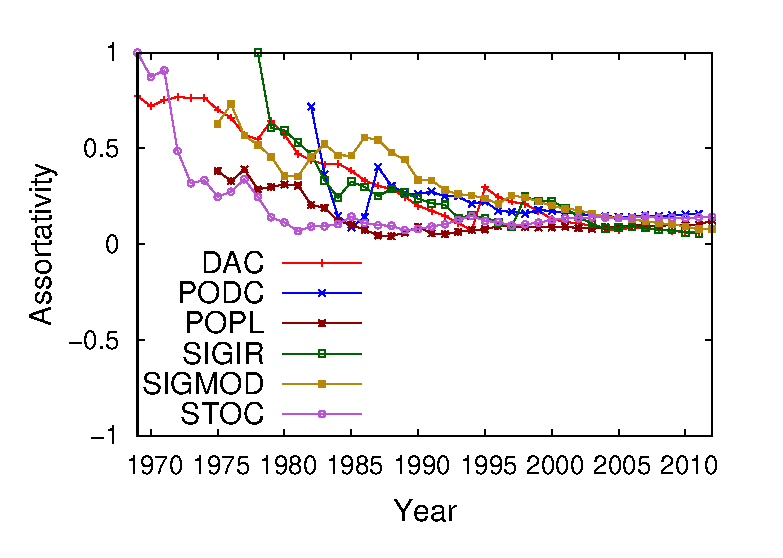
\includegraphics[scale=.33]{graficos/sigs_metricas_acumuladas_1_em_1_ano/assortatividade_grupo_temporal_web.eps}
  }%
  \subfigure[Average shortest path]{%
    \label{fig:average_shortest_path_1_in_1}
    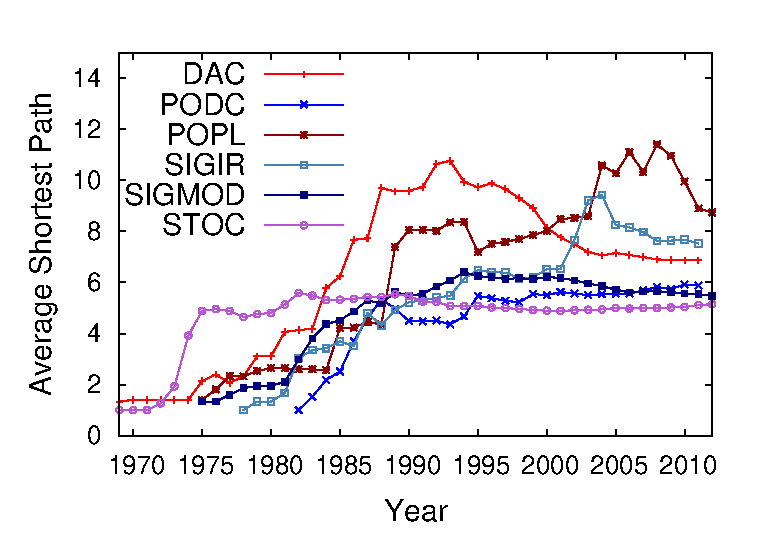
\includegraphics[scale=.33]{graficos/sigs_metricas_acumuladas_1_em_1_ano/caminho_minimo_medio_grupo_temporal_web.eps}
  }%
  \\
  \subfigure[Clustering coefficient]{%
    \label{fig:clustering_coefficient_1_in_1}
    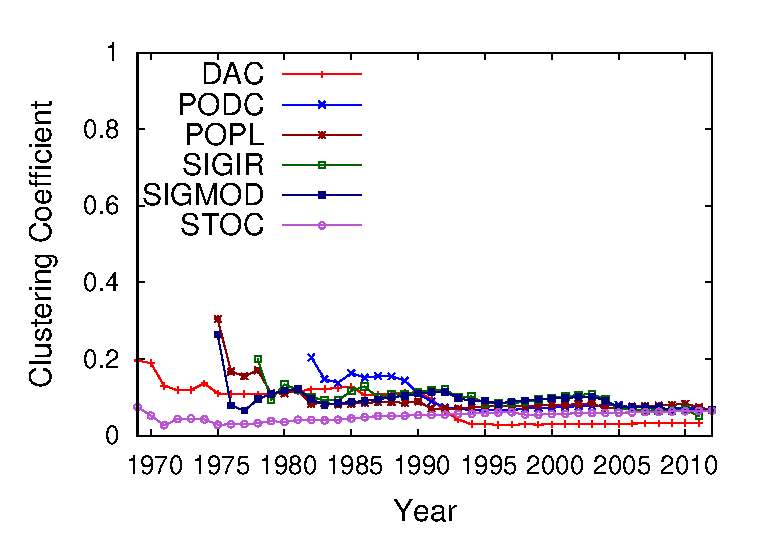
\includegraphics[scale=.33]{graficos/sigs_metricas_acumuladas_1_em_1_ano/coeficiente_agrupamento_grupo_temporal_web.eps}
  }%
  \subfigure[Largest connected component]{%
    \label{fig:largest_connected_component_1_in_1}
    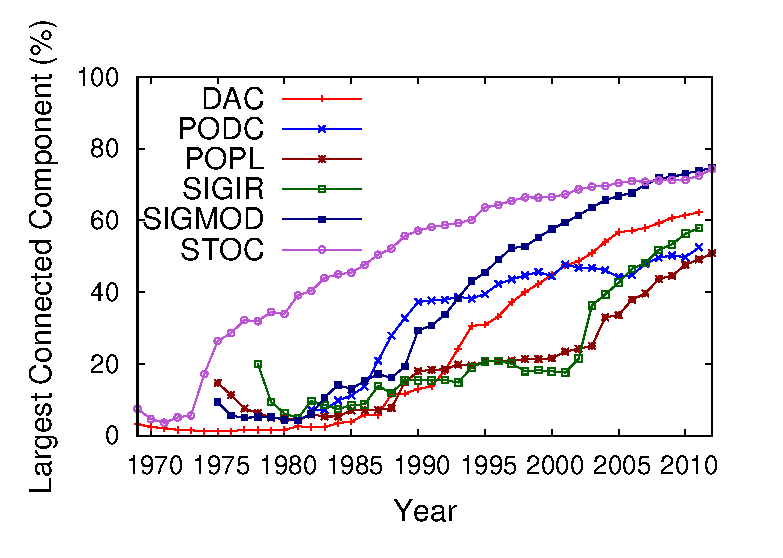
\includegraphics[scale=.33]{graficos/sigs_metricas_acumuladas_1_em_1_ano/porcentagem_maior_componente_grupo_temporal_web.eps}
  }%
  \\
  \subfigure[Average Degree - NAO CITADO NO TEXTO]{%
    \label{fig:average_degree_1_in_1}
    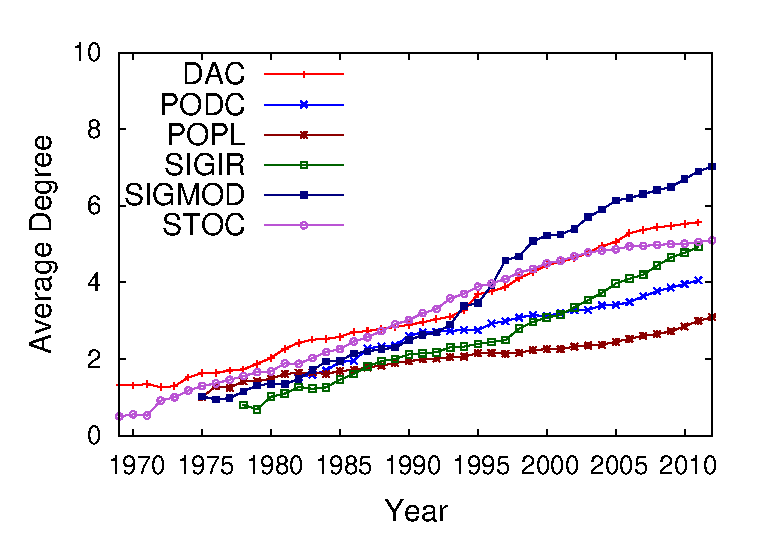
\includegraphics[scale=.33]{graficos/sigs_metricas_acumuladas_1_em_1_ano/grau_medio_nodos_grupo_temporal_web.eps}
  }%
  \end{center}
  \caption{Metrics accumulated from 1 in 1 year}
  \label{fig:metrics_accumulated_1_in_1}
\end{figure}

All in all, we can note that scientific communities have similar evolving characteristics and these properties are dynamic as they change over time.  More important, our
observations suggest that a small set authors are responsible for the social clue that create the paths among smaller and more connected research groups. Next, we seek to further
investigate this group of authors. To that end, in the next section we propose an approach to identify the author's core of scientific communities.


%\begin{figure*}
%\centering
%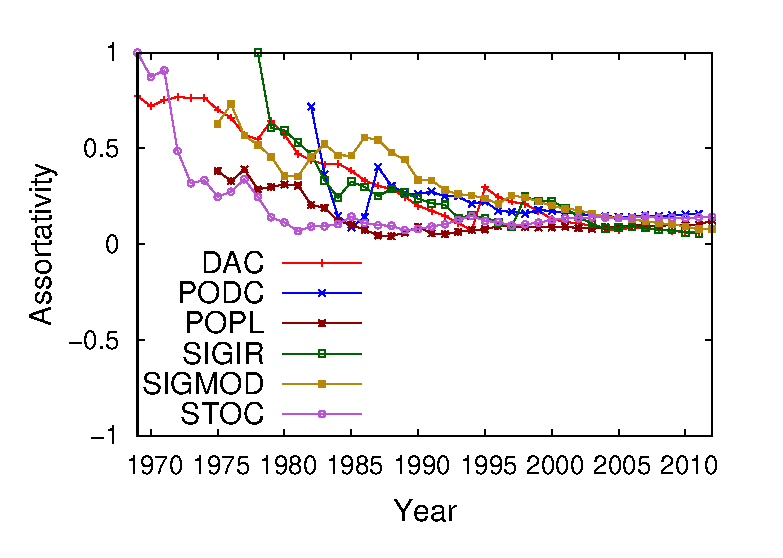
\includegraphics[scale=.4]{graficos/sigs_metricas_acumuladas_1_em_1_ano/assortatividade_grupo_temporal_web.eps}
%\caption{Assortativity accumulated from 1 in 1 year}
%\label{fig:assortativity_1_in_1}
%\end{figure*}

%\begin{figure*}
%\centering
%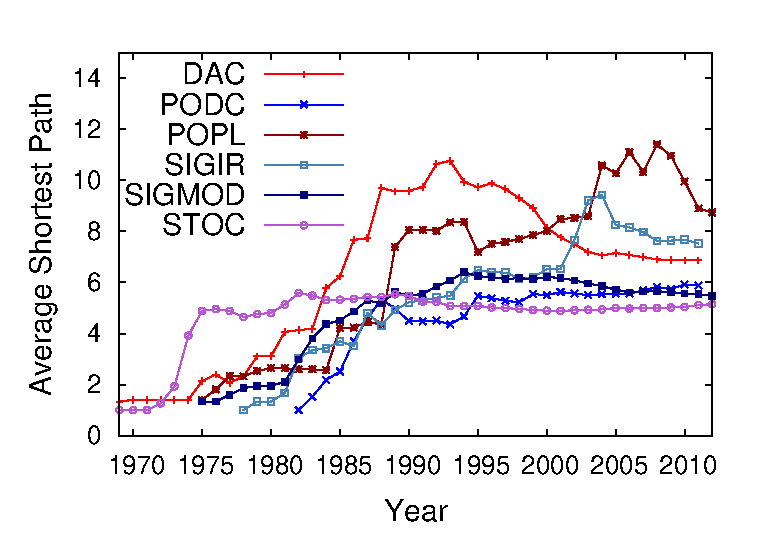
\includegraphics[scale=.4]{graficos/sigs_metricas_acumuladas_1_em_1_ano/caminho_minimo_medio_grupo_temporal_web.eps}
%\caption{Average shortest path accumulated from 1 in 1 year}
%\label{fig:average_shortest_path_1_in_1}
%\end{figure*}

%\begin{figure*}
%\centering
%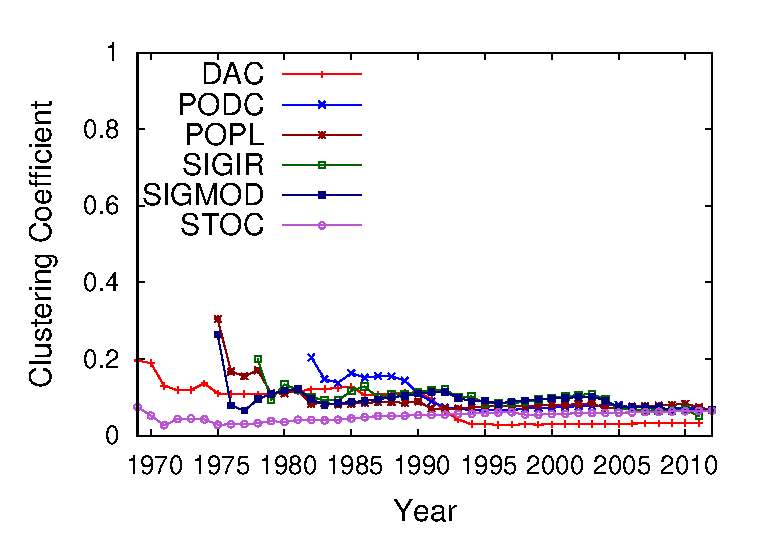
\includegraphics[scale=.4]{graficos/sigs_metricas_acumuladas_1_em_1_ano/coeficiente_agrupamento_grupo_temporal_web.eps}
%\caption{Clustering Coefficient accumulated from 1 in 1 year}
%\label{fig:clustering_coefficient_1_in_1}
%\end{figure*}

%\begin{figure*}
%\centering
%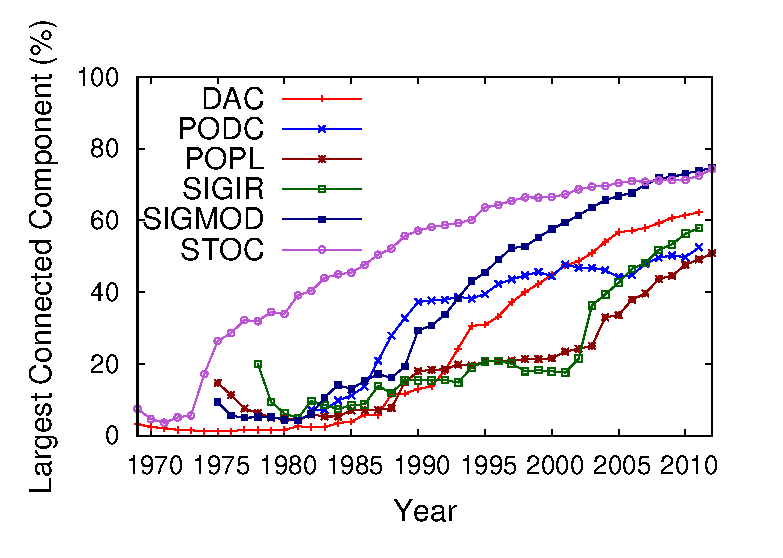
\includegraphics[scale=.4]{graficos/sigs_metricas_acumuladas_1_em_1_ano/porcentagem_maior_componente_grupo_temporal_web.eps}
%\caption{Largest connected component accumulated from 1 in 1 year}
%\label{fig:largest_connected_component_1_in_1}
%\end{figure*}



